\documentclass[10pt,a4paper]{article}

\usepackage[english]{babel}
\usepackage[utf8]{inputenc}
\usepackage[T1]{fontenc}
\usepackage[a4paper, margin=2cm]{geometry}
\usepackage{amsmath,amsfonts,amssymb}
\usepackage[colorlinks]{hyperref}
\usepackage{multicol}
\usepackage{graphicx}
\usepackage{float}
\usepackage{booktabs}

\usepackage[round]{natbib}
\bibliographystyle{abbrvnat}

\usepackage{fancyhdr}
\pagestyle{fancy}
\fancyhead[L]{02460-2026 Mini-project 2}
\fancyhead[R]{s224766, s224750, s224175 \& s224233}

% For including code
% From https://www.overleaf.com/learn/latex/Code_listing
\usepackage{listings}
\usepackage{xcolor}

\definecolor{codegreen}{rgb}{0,0.6,0}
\definecolor{codegray}{rgb}{0.5,0.5,0.5}
\definecolor{codepurple}{rgb}{0.58,0,0.82}
\definecolor{backcolour}{rgb}{0.95,0.95,0.92}

\lstdefinestyle{mystyle}{
    backgroundcolor=\color{backcolour},   
    commentstyle=\color{codegreen},
    keywordstyle=\color{magenta},
    numberstyle=\tiny\color{codegray},
    stringstyle=\color{codepurple},
    basicstyle=\ttfamily\footnotesize,
    breakatwhitespace=false,         
    breaklines=true,                 
    captionpos=b,                    
    keepspaces=true,                 
    numbers=left,                    
    numbersep=5pt,                  
    showspaces=false,                
    showstringspaces=false,
    showtabs=false,                  
    tabsize=2,
    upquote=true
}

\lstset{language=Python, style=mystyle}

\usepackage{lipsum}

\begin{document}

%%% Main text part %%%

\section*{Mini-project 2 in Advanced Machine Learning (02460)}
by Frederik Svane (s224766), Marcus Christoffersen (s224750), \\
Nicholas Larsen (s224175) \& Thor H{\o}jhus (s224233) on 01 April 2026

\begin{multicols}{2}

\subsection*{Part A: Pull-back geodesics}

We train a VAE~\citep{kingma2013vae} with a standard Gaussian prior
and a Gaussian likelihood on a 3-class subset of MNIST (2048
observations). The latent space is two-dimensional to permit
visualisation. Encoder and decoder are symmetric convolutional
networks; Gaussian noise ($\sigma\!=\!0.05$) is added to training
inputs to improve decoder smoothness, which in turn produces a
smoother pull-back metric and a better-conditioned energy landscape
for geodesic optimisation.

The pull-back metric~\citep{arvanitidis2018latent} induced by the
decoder mean $f\colon\mathcal{Z}\to\mathcal{X}$ equips the latent
space with a Riemannian structure: the metric tensor at $z$ is
$G(z) = J_f(z)^\top J_f(z)$, where $J_f$ is the decoder Jacobian.
Geodesics are shortest paths under this metric; we approximate
them by discretising a curve $c(t)$ into $N\!=\!20$ points and
minimising the energy
$\mathcal{E}(c) = \sum_{i} \lVert f(c(t_i)) - f(c(t_{i+1})) \rVert^2$
over the interior points with Adam (lr\,$=10^{-2}$, 500 steps),
keeping the endpoints fixed.

Figure~\ref{fig:geodesics_single} shows the encoded test set coloured by
digit class alongside 25 geodesics between random latent pairs.
The geodesics visibly curve away from low-density regions between
clusters: paths connecting points in different clusters bend to
follow the data manifold rather than cutting through empty space.
Within a single cluster the geodesics are nearly straight, as
expected when the decoder varies smoothly.
Across independent training runs the qualitative bending pattern
persists, but the precise paths shift because latent
representations are only identified up to rotation and
translation. Geodesics are therefore not reliable across runs:
individual paths and distances are not directly comparable,
motivating the ensemble approach in Part~B.

    \begin{figure}[H]
        \centering
        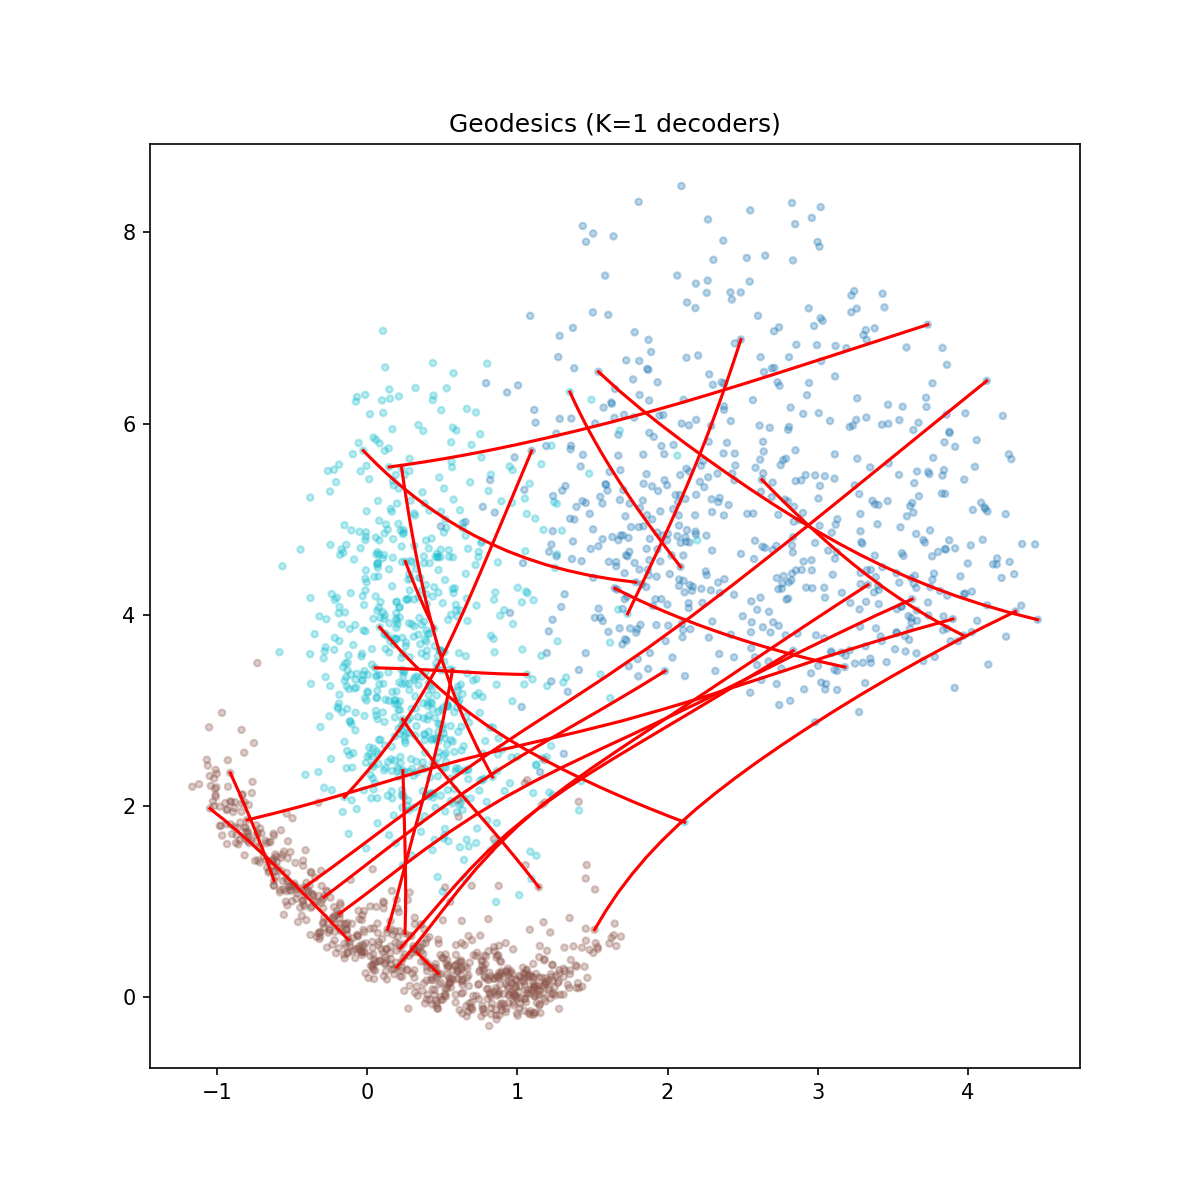
\includegraphics[width=0.7\columnwidth]{../experiment/geodesics_K1.png}
        \caption{25 pull-back geodesics ($K\!=\!1$) on the encoded test set.}
        \label{fig:geodesics_single}
    \end{figure}

    \subsection*{Part B: Ensemble VAE geometry}

    Since a single decoder's geometry is unreliable across runs, we
    replace it with a model-average geometry. All $K$ decoders share
    the same frozen encoder: the encoder and first decoder are trained
    jointly, then the encoder is fixed and $K\!-\!1$ additional decoders
    are trained independently. The model-average curve energy (eq.~1)
    is approximated via Monte Carlo: at each sample, decoder indices
    $l,k$ are drawn uniformly and the squared data-space differences
    are accumulated. The CoV (std/mean of distances across retrainings)
    measures reliability; lower is better. Geodesics minimise this
    energy with the same Adam optimiser as Part~A.

    Fig.~\ref{fig:geodesics_ensemble} shows the same 25 pairs from
    Part~A computed under $K\!=\!3$. The single-decoder paths are
    largely straight, failing to route around the low-density gap.
    With $K\!=\!3$, paths converge through the high-density corridor:
    the ensemble penalises paths through regions where decoders disagree,
    yielding geometrically consistent geodesics.
    Euclidean CoV is high (${\approx}0.23$) because latent coordinates
    vary across runs due to rotation and translation ambiguity, making
    straight-line distances unstable. Geodesic CoV (${\approx}0.12$ at
    $K\!=\!1$) is already half of this, as manifold-aware distances
    partially cancel the coordinate ambiguity. Increasing to $K\!=\!3$
    reduces it to ${\approx}0.09$: each decoder overfits its own latent
    arrangement, and averaging forces agreement on paths that are short
    across all decoders. For applications where geodesic distances
    serve as a similarity measure, $K\!=\!3$ already offers
    substantially more reliable estimates than either single-decoder
    geodesics or Euclidean distances.

    \begin{figure}[H]
        \centering
        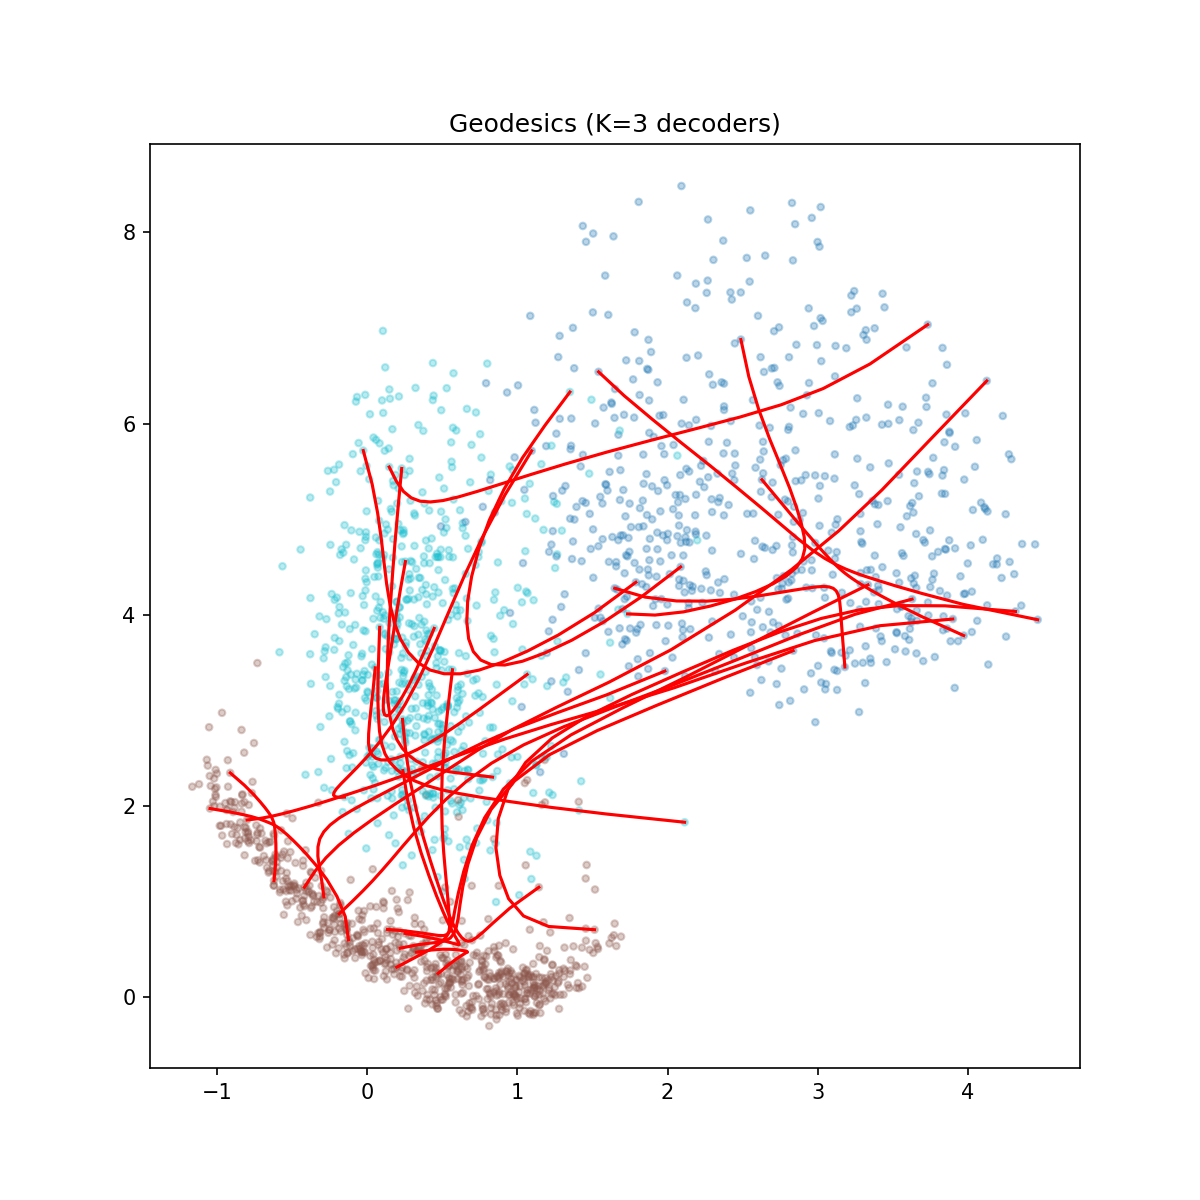
\includegraphics[height=0.45\columnwidth]{../experiment/geodesics_K3.png}
        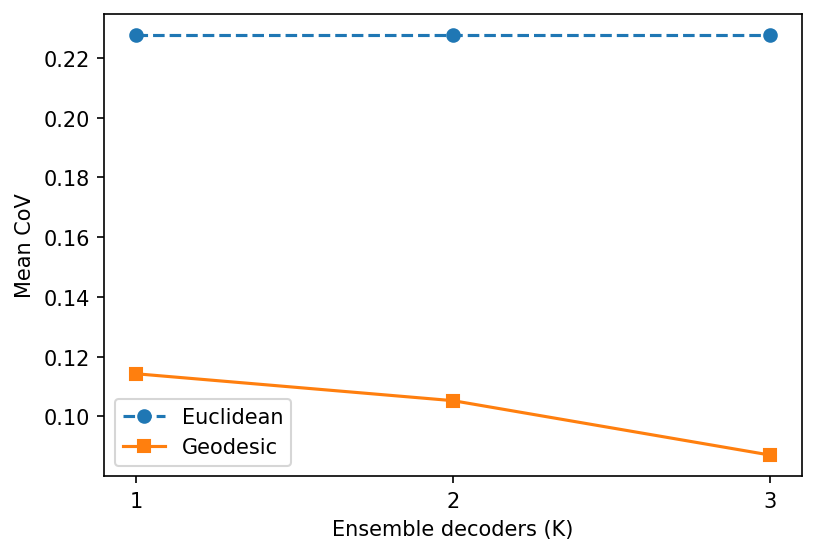
\includegraphics[height=0.40\columnwidth, width=0.4\columnwidth]{../experiment/cov_plot.png}
        \caption{Left: 25 geodesics with $K\!=\!3$ ensemble energy. Right: mean CoV vs.\ $K$ (10 pairs, 10 retrainings).}
        \label{fig:geodesics_ensemble}
    \end{figure}
\end{multicols}

\newpage

%%% Code snippet part %%%

\section*{Code snippets}

\subsection*{1. Pull-back curve energy}

\begin{lstlisting}[language=Python, caption={Curve energy (ensemble\_vae.py)}]
def curve_energy(curve, decoder):
    decoded = decoder(curve).mean
    diffs = decoded[1:] - decoded[:-1]
    return (diffs ** 2).sum()
\end{lstlisting}

\subsection*{2. Geodesic computation via energy minimisation}

\begin{lstlisting}[language=Python, caption={Geodesic optimisation (ensemble\_vae.py)}]
def compute_geodesic(a, b, decoder, num_points=20,
                     num_epochs=500, lr=1e-2):
    t = torch.linspace(0, 1, num_points,
                       device=a.device).unsqueeze(1)
    curve = (1 - t) * a + t * b
    interior = curve[1:-1].clone().detach().requires_grad_(True)
    optimizer = torch.optim.Adam([interior], lr=lr)
    for epoch in range(num_epochs):
        optimizer.zero_grad()
        full_curve = torch.cat(
            [a.unsqueeze(0), interior, b.unsqueeze(0)], dim=0)
        energy = curve_energy(full_curve, decoder)
        energy.backward()
        optimizer.step()
    with torch.no_grad():
        final_curve = torch.cat(
            [a.unsqueeze(0), interior, b.unsqueeze(0)], dim=0)
    return final_curve
\end{lstlisting}

\subsection*{3. Ensemble curve energy}

\begin{lstlisting}[language=Python, caption={Ensemble curve energy (ensemble\_vae.py)}]
def ensemble_curve_energy(curve, decoders, num_mc_samples=16):
    energy = 0.0
    for _ in range(num_mc_samples):
        l = torch.randint(len(decoders), (1,)).item()
        k = torch.randint(len(decoders), (1,)).item()
        decoded_l = decoders[l](curve[:-1]).mean
        decoded_k = decoders[k](curve[1:]).mean
        energy += (decoded_l - decoded_k).pow(2).sum()
    return energy / num_mc_samples
\end{lstlisting}

\subsection*{4. Coefficient of variation}

\begin{lstlisting}[language=Python, caption={CoV computation (ensemble\_vae.py)}]
eucl_cov = (eucl_dists.std(axis=0)
            / (eucl_dists.mean(axis=0) + 1e-8)).mean()
geod_covs = []
for K in range(1, num_decoders + 1):
    g_cov = (geod_dists[K].std(axis=0)
             / (geod_dists[K].mean(axis=0) + 1e-8)).mean()
    geod_covs.append(g_cov)
\end{lstlisting}

\newpage

%%% Bibliography %%%

\bibliography{template}

\end{document}
